\documentclass{article}

\usepackage{graphicx}
\usepackage{blindtext}
\usepackage{wrapfig}

\author{Anuj Nair}
\title{The Logic of Images and Figures in {\LaTeX}}

\begin{document}

\maketitle

Here is a Document

\begin{center}
\blindtext
\blindtext
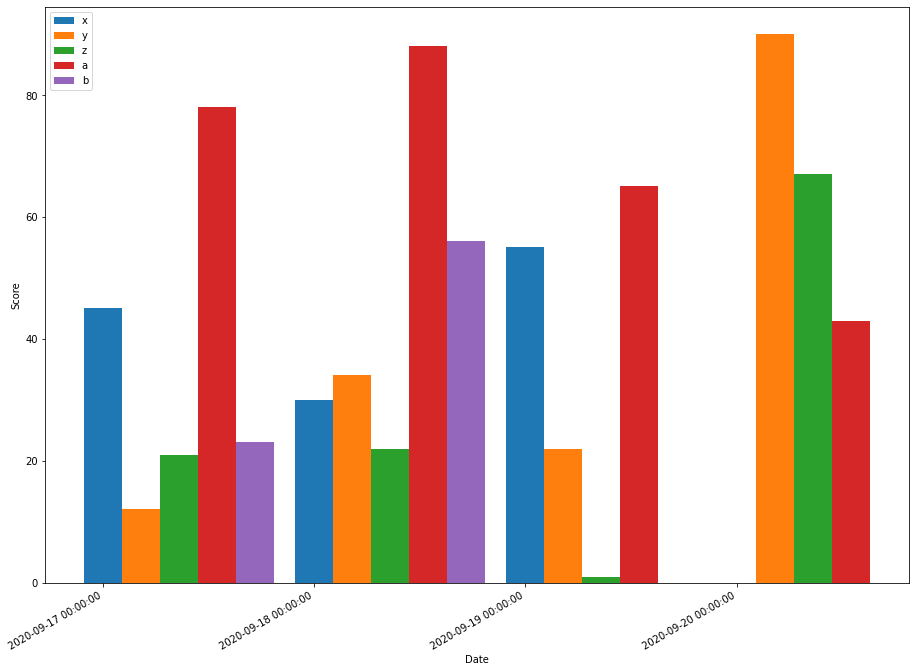
\includegraphics[width=4in,height=4in,keepaspectratio]{4_imgMng.png}
\blindtext
\end{center}
\blindtext
\blindtext
\begin{figure}[t]
\centering
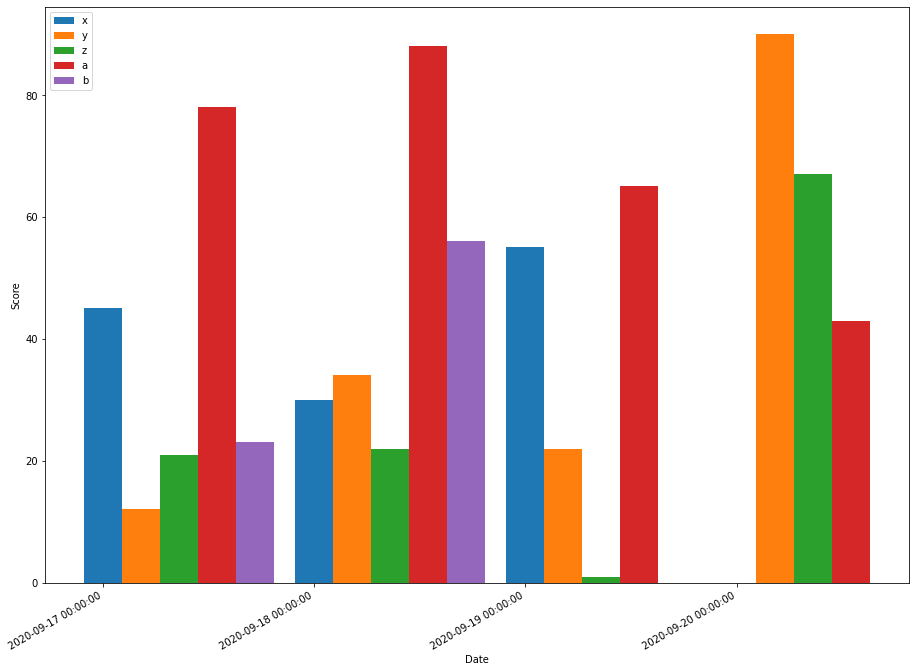
\includegraphics[scale=0.2]{4_imgMng.png}
\caption{Same graph but small}
\end{figure}
\blindtext
\blindtext
\begin{wrapfigure}{r}{3in}
\centering
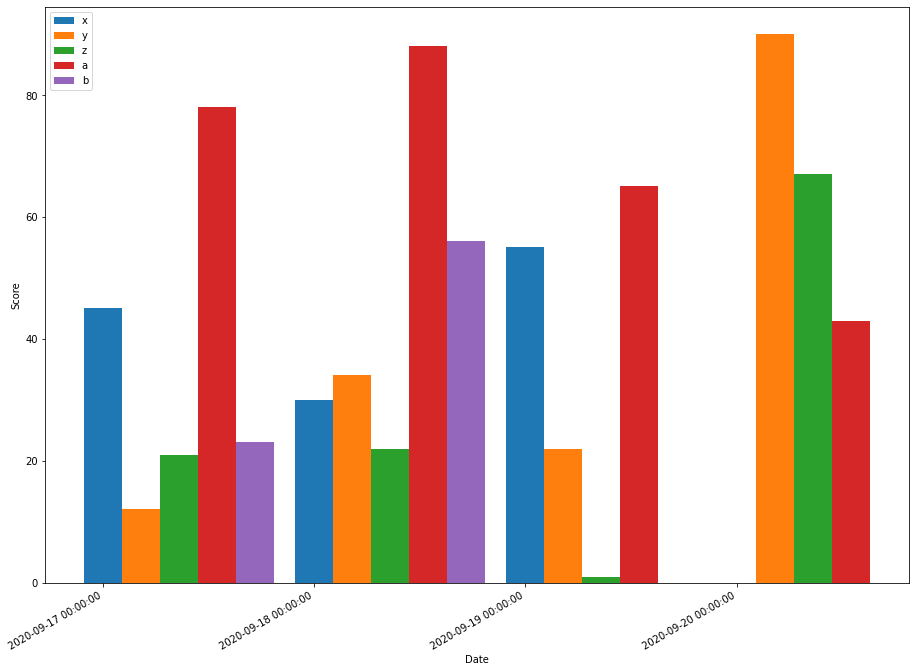
\includegraphics[width=2.5in]{4_imgMng.png}
\caption{Graph-Yasss\label{graphPic}}
\end{wrapfigure}

Please refer to Figure \ref{graphPic}
\blindtext
\begin{figure}
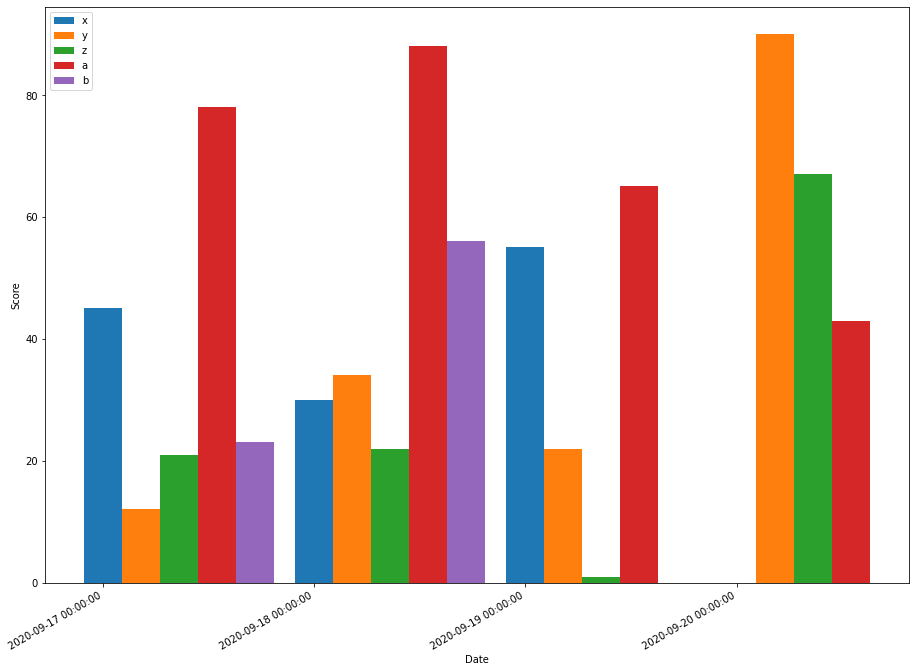
\includegraphics[width=1.1\textwidth, angle=20]{4_imgMng.png}
\caption{Same graph in 20 degree.}
\end{figure}
\blindtext

\blindtext

\blindtext


\end{document}
